
% This LaTeX was auto-generated from MATLAB code.
% To make changes, update the MATLAB code and republish this document.

\documentclass{article}
\usepackage{graphicx}
\usepackage{color}

\sloppy
\definecolor{lightgray}{gray}{0.5}
\setlength{\parindent}{0pt}

\begin{document}

    
    

\section*{19. Clenshaw--Curtis and Gauss quadrature}

\begin{verbatim}
ATAPformats
\end{verbatim}
\begin{par}
One thing that is famous about Legendre points and polynomials is their connection with \textit{Gauss quadrature}, invented by Gauss [1814]. Chebyshev points, similarly, are the basis of \textit{Clenshaw--Curtis quadrature} [Clenshaw \& Curtis 1960], and equispaced points are the basis of \textit{Newton--Cotes quadrature}.  Quadrature is the standard term for the numerical calculation of integrals.  It is one of the areas where approximation theory has an immediate link to applications, as we shall see in Theorems 19.3--19.5.
\end{par} \vspace{1em}
\begin{par}
In the basic quadrature problem, we are given a function $f\in C([-1,1])$ and wish to calculate $$ I = \int_{-1}^1 f(x) \kern 1pt dx. \eqno (19.1) $$ (More generally the integral may include a weight function $w(x)$ as in (17.1).) There is a standard idea for doing this that is the basis of the Gauss, Clenshaw--Curtis, and Newton--Cotes formulas and many others besides. Given $n\ge 0$, we sample $f$ at a certain set of $n+1$ distinct \textit{nodes} $x_0,\dots, x_n$ in $[-1,1]$.  We then approximate $I$ by $I_n$, the exact integral of the degree $n$ polynomial interpolant $p_n$ of $f$ in these nodes: $$ I_n = \int_{-1}^1 p_n(x) \kern 1pt dx. \eqno (19.2) $$ One might wonder, why use a polynomial rather than some other interpolant? This is a very good question, and in Chapter 22 we shall see that other interpolants may in fact be up to $\pi/2$ times more efficient. Nevertheless, polynomial interpolants have been the standard idea in numerical quadrature since the 18th century.
\end{par} \vspace{1em}
\begin{par}
To integrate $p_n$, we do not construct it explicitly.  Instead, $I_n$ is computed from the formula $$ I_n = \sum_{k=0}^n w_k f(x_k), \eqno (19.3) $$ where the numbers $w_0,\dots, w_n$ are a set of $n+1$ \textit{weights} that have been predetermined so that the value of $I_n$ will come out right.  From (5.1) it is clear that the weights must be the integrals of the Lagrange polynomials, $$ w_k = \int_{-1}^1 \ell_k(x) \kern 1pt dx. \eqno (19.4) $$ Another way to write (19.3) is to say that $I_n$ is given by an inner product, $$ I_n = w^T\!v, \eqno (19.5) $$ where $w$ and $v$ are column vectors of the weights $w_k$ and function values $f(x_k)$. Any linear process of computing an approximate integral from $n+1$ sample points must be representable in this inner product form, and the integration of polynomial interpolants is a linear process. The mapping from $\{f(x_k)\}$ to $I_n$ is a \textit{linear functional} (Exercise 19.1).
\end{par} \vspace{1em}
\begin{par}

When the weights $\{w_k\}$ of a quadrature formula (19.3) are determined
by the principle of integrating the polynomial interpolant, i.e.\ by
(19.4), then the formula is said to be {\em interpolatory}.  (Logically,
the term should really be {\em polynomial interpolatory}.)  For the following
theorem, we say that a formula is {\em exact} when
applied to $f$ if the result it gives is the exactly correct integral of
$f$.

\end{par} \vspace{1em}
\begin{par}
\textbf{Theorem 19.1. Polynomial degree of quadrature formulas.} \textit{For any $n\ge 0$, an $(n+1)$-point interpolatory quadrature formula such as Clenshaw--Curtis, Gauss, or Newton--Cotes is exact for $f\in {\cal P}_n$.  The $(n+1)$-point Gauss formula is exact for} $f\in {\cal P}_{2n+1}.$
\end{par} \vspace{1em}
\begin{par}
\textit{Proof.} Since an interpolatory formula is constructed by integration of a polynomial interpolant of degree $n$, it is immediate that it is exact for $f\in {\cal P}_n$. The nontrivial property to be established is that Gauss quadrature achieves more than this, being exact for polynomials all the way up to degree $2n+1$. The following standard argument, based on orthogonal polynomials, comes from [Jacobi 1826].  Gauss's original work twelve years earlier was based on continued fractions rather than orthogonal polynomials.
\end{par} \vspace{1em}
\begin{par}
Suppose that $f\in {\cal P}_{2n+1}$. Such a function can be written in the form $f(x) = P_{n+1}(x)\, q_n(x) + r_n(x)$, where $P_{n+1}$ is the $(n+1)\kern -3pt$ st Legendre polynomial and $q_n, r_n \in {\cal P}_n$. This implies $$ I =  \int_{-1}^1 f(x)\, dx  = \int_{-1}^1 P_{n+1}(x)\, q_n(x) \, dx \,+ \int_{-1}^1 r_n(x)\, dx . $$ The first of the integrals on the right is zero because of the orthogonality property of Legendre polynomials, leaving us with $$ I = \int_{-1}^1 r_n(x)\, dx. $$ Now consider $I_n$, the $(n+1)\kern -3pt$ -point Gauss quadrature approximation to $I$. The nodes of this formula are the zeros of $P_{n+1}(x)$.  Accordingly, at each node $x_k$ we have $f(x_k) = r_n(x_k)$. Thus the value $I_n$ the Gauss formula gives for $f$ will be the same as the value it gives for $r_n$.  But $r_n\in {\cal P}_n$, so this value is exactly the integral of $r_n$, that is, $I_n = I$. $~\hbox{\vrule width 2.5pt depth 2.5 pt height 3.5 pt}$
\end{par} \vspace{1em}
\begin{par}
Theorem 19.1 is famous, but we shall see that it is misleading.  It suggests that there is a significant gap between Clenshaw--Curtis and Newton--Cotes quadrature, with one rate of convergence, and Gauss quadrature, with a rate twice as high.  In fact, the great gap is between Newton--Cotes, which does not converge at all in general, and both Clenshaw--Curtis and Gauss, which converge for every continuous $f$ and do so typically at similar rates.
\end{par} \vspace{1em}
\begin{par}

First, let us give some more details of the Clenshaw--Curtis and
Gauss formulas.  For
Clenshaw--Curtis quadrature, one way to compute $I_n$ is by constructing
the weight vector $w$ explicitly. It can be shown that the weights are
all positive and sum to 2 (the same properties also hold for Gauss
quadrature weights, whose computation we discuss later in the chapter).
From a practical point of view, this approach may be advantageous for
integrating a collection of functions on a single Chebyshev grid. There
is a classical formula for calculation of the weights with $O(n^2)$
operations [Davis \& Rabinowitz 1984, Trefethen 2000], and it is also
possible to compute the weights faster, in $O(n\log n)$ operations, using
the FFT [Waldvogel 2006].  This fast algorithm is invoked by Chebfun when
the command {\tt chebpts} is called with two arguments, as we illustrate with
$n+1=3$:

\end{par} \vspace{1em}
\begin{par}
 \vskip -2em 
\end{par} \vspace{1em}
\begin{verbatim}
[nodes,weights] = chebpts(3)
\end{verbatim}

        \color{lightgray} \begin{verbatim}nodes =
    -1
     0
     1
weights =
   0.333333333333333   1.333333333333333   0.333333333333333
\end{verbatim} \color{black}
    \begin{par}
 \vskip 1pt 
\end{par} \vspace{1em}
\begin{par}
By increasing $3$ to one million we see the speed of Waldvogel's algorithm:
\end{par} \vspace{1em}
\begin{par}
 \vskip -2em 
\end{par} \vspace{1em}
\begin{verbatim}
tic, [nodes,weights] = chebpts(1000000); toc
\end{verbatim}

        \color{lightgray} \begin{verbatim}Elapsed time is 0.111820 seconds.
\end{verbatim} \color{black}
    \begin{par}
 \vskip 1pt 
\end{par} \vspace{1em}
\begin{par}
The other way to carry out Clenshaw--Curtis quadrature, simplest when just one or a small number of integrands are involved, is to use the FFT to transform the problem to coefficient space (see Chapter 3) at a cost of $O(n \log n)$ operations per integrand.  (This idea was not proposed by Clenshaw and Curtis, who wrote before the rediscovery of the FFT in 1965, but by Morven Gentleman a few years later [Gentleman 1972a, 1972b].)  To see how this works, we observe that the integral of the Chebyshev polynomial $T_k$ from $-1$ to $1$ is zero if $k$ is odd and $$ \int_{-1}^1 T_k(x)\, dx = {2\over 1-k^2} \eqno (19.6) $$ if $k$ is even (Exercise 19.6). This gives us the following theorem, the basis of the FFT realization of Clenshaw--Curtis quadrature:
\end{par} \vspace{1em}
\begin{par}
\textbf{Theorem 19.2. Integral of a Chebyshev series.} \textit{The integral of a degree $n$ polynomial expressed as a Chebyshev series is} $$ \int_{-1}^1\; \sum_{k=0}^n c_k T_k(x)\, dx \;= \sum_{k=0,\,k\kern 1pt\hbox{\footnotesize even}}^n {2c_k\over 1-k^2} . $$ \textit{Proof.} Follows from (19.6). $~\hbox{\vrule width 2.5pt depth 2.5 pt height 3.5 pt}$
\end{par} \vspace{1em}
\begin{par}
Chebfun applies Theorem 19.2 every time one types \texttt{sum(f)}, and this theorem is also the basis of Waldvogel's algorithm mentioned above.
\end{par} \vspace{1em}
\begin{par}
By combining (19.6) with Theorems 8.1 and 19.1, we can now write down a theorem about the geometric convergence of Clenshaw--Curtis and Gauss quadrature for analytic integrands. For Gauss quadrature, this estimate is due to Rabinowitz [1969], and the extension to Clenshaw--Curtis can be found in [Trefethen 2008]. This result is fundamental and very important. \textit{For analytic integrands, the Gauss and Clenshaw--Curtis formulas converge geometrically.} Every numerical analysis textbook should state this fact.
\end{par} \vspace{1em}
\begin{par}
\textbf{Theorem 19.3. Quadrature formulas for analytic integrands.} \textit{Let a function $f$ be analytic in $[-1,1]$ and analytically continuable to the open Bernstein ellipse} $E_\rho,$ \textit{where it satisfies $|f(z)|\le M$ for some $M$.  Then $(n+1)\kern -3pt$ -point Clenshaw--Curtis quadrature with $n\ge 2$ applied to $f$ satisfies} $$ |I-I_n| \le {64\over 15}{M\rho^{1-n}\over \rho^2-1} \eqno (19.7) $$ \textit{and $(n+1)\kern -3pt$ -point Gauss quadrature with $n\ge 1$ satisfies} $$ |I-I_n| \le {64\over 15} {M \rho^{-2n}\over \rho^2-1}. \eqno (19.8) $$ \textit{The factor $\rho^{1-n}$ in $(19.7)$ can be improved to $\rho^{-n}$ if $n$ is even, and the factor $64/15$ can be improved to $144/35$ if $n\ge 4$ in $(19.7)$ or $n\ge 2$ in $(19.8)$.}
\end{par} \vspace{1em}
\begin{par}
\textit{Proof.} If the constants $64/15$ are increased to $8$ and $\rho^2-1$ is reduced to $\rho-1$, these conclusions can be obtained as corollaries of Theorem 8.2. The key is to note that that the error in integrating $f$ will be the same as the error in integrating $f-f_n$.  Applying the triangle inequality, this gives us $$ |I-I_n| \le |I(f-f_n)| + |I_n(f-f_n)|. $$ By Theorem 8.2, $|(f- f_n)(x)| \le 2M\rho^{-n}/(\kern .7pt\rho-1)$ for each $|x|$.  Since the interval $[-1,1]$ has length $2$, this implies $$ |I(f-f_n)| \le {4M\rho^{-n}\over \rho-1}. $$ In addition to this, there also holds the analogous property $$ |I_n(f-f_n)| \le { 4M\rho^{-n}\over \rho-1}. $$ This follows from the fact that the weights are positive.
\end{par} \vspace{1em}
\begin{par}
To get the sharper results stated, we use an additional fact: both Gauss and Clenshaw--Curtis formulas get the right answer when integrating an odd function, namely zero. In particular the error is zero in integration of $T_k(x)$ for any odd $k$. Now by Theorem 19.1, Gauss quadrature is exact through the term of degree $2n+1$ in the Chebyshev expansion of $f$.  Since odd terms do not contribute, we see that the error in integrating $f$ by $(n+1)$-point Gauss quadrature will thus be the error in integrating $$ a_{2n+2}^{} T_{2n+2}^{}(x) + a_{2n+4}^{} T_{2n+4}^{}(x) + \dots , $$ a series in which the smallest index that appears is at least $4$. Now by (19.6), the true integral of $T_k$ for $k\ge 4$ is at most $2/15$. When $T_k$ is integrated over $[-1,1]$ by the Gauss quadrature formula, the result will be at most $2$ since the weights are positive and add up to 2.  Thus the error in integrating each $T_k$ is at most $2 + 2/15 = 32/15$. Combining this estimate with the bound $|a_k|\le 2M\rho^{-k}$ of Theorem 8.1 gives (19.8).  The argument for (19.7) is analogous.  For the improvement from 64/15 to 144/35, see Exercise 19.5. $~\hbox{\vrule width 2.5pt depth 2.5 pt height 3.5 pt}$
\end{par} \vspace{1em}
\begin{par}
Just as Theorem 19.3 follows from the results of Chapter 8 for analytic integrands, there is an analogous result for differentiable integrands based on the results of Chapter 7.
\end{par} \vspace{1em}
\begin{par}

{\em {\bf Theorem 19.4. Quadrature formulas for differentiable integrands.}
For any $f\in C([-1,1])$, both the Clenshaw--Curtis and Gauss approximations
$I_n$ converge to the integral $I$ as $n\to\infty$.
For an integer $\nu \ge 1$, let $f$ and its derivatives through $f^{(\nu-1)}$
be absolutely continuous on $[-1,1]$
and suppose the $\nu$th derivative $f^{(\nu )}$ is of bounded
variation $V$.   Then $(n+1)\kern -3pt$ -point
Clenshaw--Curtis quadrature applied to $f$ satisfies
$$ |I-I_n| \le {32\over 15}{V \over \pi \nu (n-\nu)^\nu} \eqno (19.9) $$
for $n>\nu$ and $(n+1)\kern -3pt$ -point Gauss quadrature satisfies
$$ |I-I_n| \le {32\over 15}{V \over \pi \nu (n-2\nu-1)^{2\nu+1}} \eqno (19.10) $$
for $n>2\nu+1$.}

\end{par} \vspace{1em}
\begin{par}
\textit{Proof.} The first assertion, for arbitrary continuous $f$, is due to Stieltjes [1884].  As for (19.9) and (19.10), these can be derived as in the previous proof, but now using Theorem 7.2. $~\hbox{\vrule width 2.5pt depth 2.5 pt height 3.5 pt}$
\end{par} \vspace{1em}
\begin{par}
Here is a numerical example, the integration of the function (18.1) with a sequence of spikes: $$ I = \int_{-1}^1 e^x \kern 1pt [\hbox{sech}(4\sin(40x))]^{\exp(x)} \kern 1pt dx \eqno (19.11) $$
\end{par} \vspace{1em}
\begin{par}
 \vskip -3em 
\end{par} \vspace{1em}
\begin{verbatim}
ff = @(x) exp(x).*sech(4*sin(40*x)).^exp(x);
x = chebfun('x'); f = ff(x);
FS = 'fontsize';
clf, plot(f), grid on, title('The spiky integrand (19.11)',FS,9)
\end{verbatim}

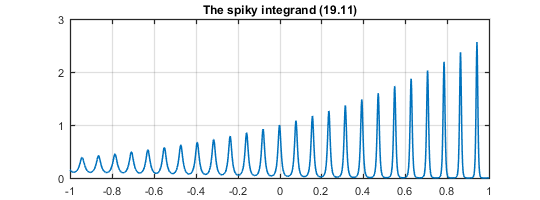
\includegraphics [width=4in]{chap19_01.png}
\begin{par}
 \vskip 1pt 
\end{par} \vspace{1em}
\begin{par}
The corresponding chebfun is not exactly short:
\end{par} \vspace{1em}
\begin{par}
 \vskip -2em 
\end{par} \vspace{1em}
\begin{verbatim}
length(f)
\end{verbatim}

        \color{lightgray} \begin{verbatim}ans =
        3680
\end{verbatim} \color{black}
    \begin{par}
Nevertheless, Chebfun computes its integral to 15 digits of accuracy in a fraction of a second:
\end{par} \vspace{1em}
\begin{par}
 \vskip -2em 
\end{par} \vspace{1em}
\begin{verbatim}
sum(f)
\end{verbatim}

        \color{lightgray} \begin{verbatim}ans =
   0.543384000907901
\end{verbatim} \color{black}
    \begin{par}
Now let us look at Gauss quadrature. The nodes for the $n+1$-point Gauss formula are the roots of the Legendre polynomial $P_{n+1}(x)$.  A good method for computing these numbers is implicit in Theorem 18.1 and the comment after it.  According to that theorem, the roots of a polynomial expressed as a Chebyshev series are equal to the eigenvalues of a colleague matrix whose structure is tridiagonal apart from a nonzero final row. If the Chebyshev series reduces to the single polynomial $T_{n+1}$, the matrix reduces to tridiagonal without the extra row. Similarly the roots of a polynomial expressed as a series in Legendre polynomials are the eigenvalues of a comrade matrix, which is again tridiagonal except for a final row, and for the roots of $P_{n+1}$ itself, the matrix reduces to tridiagonal.  When symmetrized, this matrix is called a \textit{Jacobi matrix} (Exercise 19.7). The classic numerical algorithm for implementing Gauss quadrature formulas comes from Golub and Welsch in 1969, who showed that the weights as well as the nodes can be obtained by solving the eigenvalue problem for this Jacobi matrix [Golub \& Welsch 1969]. The Golub--Welsch algorithm can be coded in six lines of Matlab (see \texttt{gauss.m} in [Trefethen 2000]), and the operation count is in principle $O(n^2)$, although it is $O(n^3)$ in the simple implementation since Matlab does not offer a command to exploit the tridiagonal structure of the eigenvalue problem.
\end{par} \vspace{1em}
\begin{par}
For larger values of $n$, a much faster alternative algorithm was introduced by Glaser, Liu, and Rokhlin [2007], based on numerical solution of certain linear ordinary differential equations by high-order Taylor series approximations combined with Newton iteration.  This GLR algorithm shrank the operation count dramatically to $O(n)$ and became the default algorithm invoked by Chebfun during 2009--2012 when the \texttt{legpts} command is called with two output arguments. Most recently an even faster algorithm has been introduced by Hale and Townsend [2012], which is Chebfun's default at the time of this writing. The key idea of the Hale--Townsend algorithm is to start from high accuracy asymptotic approximations for nodes and then take one or two Newton steps, with $P_n$ and $P_n'$ evaluated to machine precision by known asymptotic formulas.  When $n$ is large enough, one may not even need any Newton steps at all.  A crucial feature is that the method treats the nodes independently, so that it vectorizes readily, and this is a primary reason why it is approximately 20 times faster than the GLR algorithm in a Matlab implementation.
\end{par} \vspace{1em}
\begin{par}
Following the illustration of Clenshaw--Curtis quadrature earlier, here are nodes and weights for Gauss quadrature with $n+1=3$:
\end{par} \vspace{1em}
\begin{par}
 \vskip -2em 
\end{par} \vspace{1em}
\begin{verbatim}
[nodes,weights] = legpts(3)
\end{verbatim}

        \color{lightgray} \begin{verbatim}nodes =
  -0.774596669241483
                   0
   0.774596669241483
weights =
   0.555555555555556   0.888888888888889   0.555555555555556
\end{verbatim} \color{black}
    \begin{par}
 \vskip 1pt 
\end{par} \vspace{1em}
\begin{par}
And here is the time it takes to compute Gauss quadrature nodes and weights for one million points, not much slower than Clenshaw--Curtis:
\end{par} \vspace{1em}
\begin{par}
 \vskip -2em 
\end{par} \vspace{1em}
\begin{verbatim}
tic, [nodes,weights] = legpts(1000000); toc
\end{verbatim}

        \color{lightgray} \begin{verbatim}Elapsed time is 0.159500 seconds.
\end{verbatim} \color{black}
    \begin{par}
 \vskip 1pt 
\end{par} \vspace{1em}
\begin{par}
For example, here is the integral (19.11) computed by $n$-point Gauss quadrature for various values of $n$. We write \texttt{w*gg(s)} rather than \texttt{w'*gg(s)} since $w$ as returned by \texttt{legpts} is a row vector, not a column vector.
\end{par} \vspace{1em}
\begin{par}
 \vskip -2em 
\end{par} \vspace{1em}
\begin{verbatim}
for n = 500:500:2000
  tic
  [s,w] = legpts(n+1);
  I = w*ff(s); t = toc;
  fprintf('n = %4d,  I = %16.14f,  time = %6.4f\n',n,I,t)
end
\end{verbatim}

        \color{lightgray} \begin{verbatim}n =  500,  I = 0.54339275810622,  time = 0.0086
n = 1000,  I = 0.54338400182558,  time = 0.0140
n = 1500,  I = 0.54338400090784,  time = 0.0050
n = 2000,  I = 0.54338400090790,  time = 0.0069
\end{verbatim} \color{black}
    \begin{par}
Gauss quadrature has not often been employed for numbers of nodes in the thousands, because with traditional algorithms the computations are too expensive.  It is clear from this experiment that the GLR and Hale--Townsend algorithms make such computations feasible after all.
\end{par} \vspace{1em}
\begin{par}
So is Gauss quadrature the formula of choice?  In particular, how does it compare with Clenshaw--Curtis quadrature as $n\to\infty$? As mentioned above, the traditional expectation, based on Theorem 19.1 and seemingly supported by Theorems 19.3 and 19.4, is that Gauss should converge twice as fast as Clenshaw--Curtis. However, numerical experiments show that the truth is not so simple. We begin with the easy integrand $f(x) = \exp(-100x^2)$.
\end{par} \vspace{1em}
\begin{par}
 \vskip -2em 
\end{par} \vspace{1em}
\begin{verbatim}
gg = @(x) exp(-100*x.^2);
I = sum(chebfun(gg));
errcc = []; errgauss = [];
nn = 2:2:80;
for n = nn
   Icc = sum(chebfun(gg,n+1));
   errcc = [errcc abs(I-Icc)];
   [s,w] = legpts(n+1);
   Igauss = w*gg(s);
   errgauss = [errgauss abs(I-Igauss)];
end
hold off, semilogy(nn,errcc,'.-','markersize',10), grid on
hold on, semilogy(nn,errgauss,'h-m','markersize',4), grid on
title('Gauss vs. Clenshaw-Curtis quadrature',FS,9)
\end{verbatim}

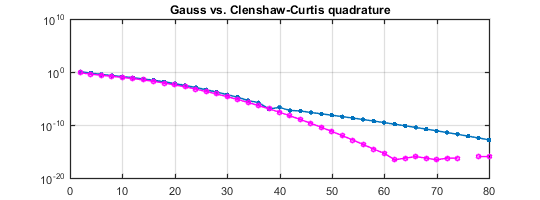
\includegraphics [width=4in]{chap19_02.png}
\begin{par}
 \vskip 1pt 
\end{par} \vspace{1em}
\begin{par}

This behavior is typical: for smaller values of $n$, Clenshaw--Curtis
(dots) and Gauss quadrature (stars) have similar accuracy, not a
difference of a factor of~2.  This effect was pointed out by Clenshaw and
Curtis in their original paper [1960].  Only at a sufficiently large
value of $n$, if the integrand is analytic, does a kink appear in the
Clenshaw--Curtis convergence curve, whose further convergence is then
about half as fast as before.   An explanation of this effect based on
ideas of rational approximation is given in Figures 4--6 of [Trefethen
2008], and another explanation based on aliasing can be derived from
Theorems 4.2 and 19.2 and goes back to O'Hara and Smith [1968] (Exercise
19.4). For a full analysis, see [Weideman \& Trefethen 2007].

\end{par} \vspace{1em}
\begin{par}
Here is a similar comparison for the harder integral (19.11):
\end{par} \vspace{1em}
\begin{par}
 \vskip -2em 
\end{par} \vspace{1em}
\begin{verbatim}
I = sum(f);
errcc = []; errgauss = []; tcc = []; tgauss = [];
nn = 50:50:2000;
for n = nn
   tic, Icc = sum(chebfun(ff,n+1)); t = toc;
   tcc = [tcc t]; errcc = [errcc abs(I-Icc)];
   tic, [s,w] = legpts(n+1); t = toc;
   Igauss = w*ff(s);
   tgauss = [tgauss t]; errgauss = [errgauss abs(I-Igauss)];
end
hold off, semilogy(nn,errcc,'.-','markersize',10), grid on
hold on, semilogy(nn,errgauss,'h-m','markersize',4)
title('Gauss vs. Clenshaw-Curtis quadrature',FS,9)
\end{verbatim}

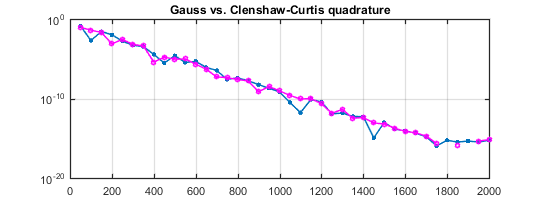
\includegraphics [width=4in]{chap19_03.png}
\begin{par}
 \vskip 1pt 
\end{par} \vspace{1em}
\begin{par}
This time, for the values of $n$ under study, the kink does not appear at all.  Clenshaw--Curtis has approximately the same accuracy as Gauss throughout, and in particular, it obtains the correct integral to machine precision by around $n=1800$, which is about half the length of the chebfun, \texttt{length(f)}, reported earlier! This is typical of Clenshaw--Curtis quadrature: just as with Gauss quadrature, the quadrature value often converges about twice as fast as the underlying polynomial approximation, even though Theorems 19.1, 19.3, and 19.4 give no hint of such behavior.
\end{par} \vspace{1em}
\begin{par}
There is a theorem that substantiates this effect. The following result, whose proof we shall not give, comes from [Trefethen 2008].
\end{par} \vspace{1em}
\begin{par}
\textbf{Theorem 19.5. Clenshaw--Curtis quadrature for differentiable integrands.} \textit{Under the hypotheses of Theorem $19.4$, the same conclusion $(19.10)$ also holds for $(n+1)$-point Clenshaw--Curtis quadrature:} $$ |I-I_n| \le {32\over 15} {V \over \pi \nu (n-2\nu-1)^{2\nu+1}}. \eqno (19.12) $$ \textit{The only difference is that this bound applies for all sufficiently large $n$ (depending on $\nu$ but not $f$) rather than for $n>2\nu+1$.}
\end{par} \vspace{1em}
\begin{par}
\textit{Proof.} See [Trefethen 2008]. Here, the definition of $V$ is somewhat different from the one in [Trefethen 2008], but this does not affect the argument leading to (19.12). $~\hbox{\vrule width 2.5pt depth 2.5 pt height 3.5 pt}$
\end{par} \vspace{1em}
\begin{par}
All in all, though Gauss quadrature is more celebrated than Clenshaw--Curtis, and certainly has some beautiful properties, its behavior in practice is often not very much different.
\end{par} \vspace{1em}
\begin{par}
For an extensive survey of many aspects of Gauss quadrature, see [Gautschi 1981], and for general information about numerical integration, see [Davis \& Rabinowitz 1984]. In practical applications and software implementations it is common to use adaptive formulas of low or moderate order rather than letting $n$ increase toward $\infty$ with a global grid, though Chebfun is an exception to this pattern.
\end{par} \vspace{1em}
\begin{par}
As mentioned earlier, both Gauss and Clenshaw--Curtis quadrature grids can be improved by a factor approaching $\pi/2$ by the introduction of a change of variables, taking us beyond the realm of polynomial approximations.  These ideas are discussed in Chapter 22.
\end{par} \vspace{1em}
\begin{par}
We have not said much about Newton--Cotes quadrature formulas, based on equispaced points.  For smaller orders these are of practical interest: $n=4$ gives \textit{Simpson's rule}, and Espelid has used Newton--Cotes rules of order up to 33 as the basis of excellent codes \texttt{coted2a} and \texttt{da2glob} for adaptive quadrature [Espelid 2004].  The weights $\{w_j\}$ of Newton--Cotes formula, however, oscillate in sign between magnitudes on the order of $2^n$, a reflection of the Runge phenomenon, causing terrible numerical instability for large $n$.  Even in the absence of rounding errors, the results of Newton--Cotes formulas do not converge in general as $n\to\infty$, even for analytic functions.  It was clear upon publication of Runge's paper in 1901 that such divergence was likely, and a theorem to this effect was proved by $\hbox{P\'olya}$ [1933].
\end{par} \vspace{1em}
\begin{par}
We close this chapter by mentioning an elegant application of Gauss quadrature nodes and weights pointed out by Wang and Xiang [2012].
\end{par} \vspace{1em}
\begin{par}
\textbf{Theorem 19.6. Barycentric weights for Legendre points.} \textit{Let the numbers $\lambda_0, \dots , \lambda_k$ be defined by $$ \lambda_k = (-1)^k \sqrt{(1-x_k^2) w_k}, \eqno (19.13) $$ where $\{x_k\}$ and $\{w_k\}$ are the nodes and weights for $(n+1)$-point Gauss quadrature.  If these numbers are taken as weights in the barycentric formula $(5.11)$, they yield the polynomial interpolant through Legendre points.}
\end{par} \vspace{1em}
\begin{par}
 \vspace{-1em} 
\end{par} \vspace{1em}
\begin{par}
\textit{Proof.} See Theorem 3.1 of [Wang \& Xiang 2012]. $~\hbox{\vrule width 2.5pt depth 2.5 pt height 3.5 pt}$
\end{par} \vspace{1em}
\begin{par}
In view of the Glaser--Liu--Rokhlin algorithm for Gauss quadrature, this theorem implies that polynomial interpolants in Legendre points, like Chebyshev points, can be evaluated in $O(n)$ operations. The formulas are implemented in Chebfun and accessed when one calls \texttt{legpts}, \texttt{jacpts}, \texttt{hermpts} or \texttt{lagpts} with three output arguments [Hale \& Trefethen 2012].
\end{par} \vspace{1em}
\begin{par}

\begin{displaymath}
\framebox[4.7in][c]{\parbox{4.5in}{\vspace{2pt}\sl
{\sc Summary of Chapter 19.}
Clenshaw--Curtis quadrature is derived by interpolating a polynomial
interpolant in Chebyshev points, and Gauss quadrature from Legendre
points.  The nodes and weights for both families can be computed quickly
and accurately, even for millions of points. Though Gauss has twice the
polynomial order of accuracy of Clenshaw--Curtis, their rates of
convergence are approximately the same for non-analytic
integrands.\vspace{2pt}}}
\end{displaymath}

\end{par} \vspace{1em}
\begin{par}
 \smallskip\small\parskip=2pt
\par
{\bf Exercise 19.1.  Riesz Representation Theorem.}
(a) Look up the Riesz Representation Theorem and write down a careful
mathematical statement of it .  (b) Show that the computation of an
approximate integral $I_n$ from $n+1$ samples of a function $f\in
C([-1,1])$ by integrating the degree $n$ polynomial interpolant through a
fixed set of $n+1$ nodes in $[-1,1]$ is an example of the kind of linear
functional to which this theorem applies, provided we work in a
finite-dimensional space rather than all of $C([-1,1])$.
(c) In what sense is the Riesz Representation Theorem significantly more
general than is needed for this particular application to quadrature?
\par
{\bf Exercise 19.2.  quad, quadl, quadgk.}
Evaluate (19.11) with Matlab's {\tt quad}, {\tt quadl}, and {\tt quadgk}
commands. As a function of the specified precision, what is the actual
accuracy obtained and how long does the computation take?  How do these
results compare with Chebfun {\tt sum}?
\par
{\bf Exercise 19.3.  Quadrature weights.}
(a) Use Chebfun to illustrate the identity (19.4) for Clenshaw--Curtis
quadrature in the case $n = 20$, $k=7$.
(b) Do the same for Gauss quadrature.
\par
{\bf Exercise 19.4.  Accuracy of Clenshaw--Curtis quadrature.}
(a) Using theorems of Chapters 4 and 19, derive an exact expression for
the error $I-I_n$ in Clenshaw--Curtis quadrature applied to the function $f(x) =
T_k(x)$ for $k> n$.  (b) [to be continued.  See eqs (9) and (9') of
Gentleman [1972a].]
\par
{\bf Exercise 19.5.  Sharpening Theorem 19.3.}  Suppose
we assume $n\ge 2$ instead of $n\ge 1$ in the Gauss quadrature bound
of Theorem 19.3.  Show why the constant $64/15$ improves to
$144/35$.  What is this actual ``constant'' as a function of $n$?
\par
{\bf Exercise 19.6.  Integral of a Chebyshev polynomial.}
Derive the formula (19.6) for the integral of $T_k(x)$ with $k$
even.  (Hint: Following the proof of Theorem 3.1,
replace $T_k(x) dx$ by $(z^k+z^{-k})(dx/dz) dz$.)
\par
{\bf Exercise 19.7.  Symmetrization in the Golub--Welsch algorithm.}
The nodes $\{x_j\}$ of the $(n+1)$-point Gauss quadrature rule are
the zeros of the Legendre polynomial $P_{n+1}$.  From the recurrence
relation (17.6), it follows as in Theorem 18.1 that they are the
eigenvalues of the $(n+1)\times(n+1)$ tridiagonal matrix with zeros
on the main diagonal, [xxx] on the first superdiagonal, and [xxx] on the first
subdiagonal.  Find the unique diagonal matrix $D = \hbox{diag}\kern.7pt (d_0,\dots,d_n)$
with $d_0=1$ and $d_j>0$ for $j\ge 1$ such that $B = D A D^{-1}$, which has the
same eigenvalues as $A$, is real symmetric.  What are the
entries of $B$?  (This symmetrized matrix is the Jacobi matrix that is
the basis of the Golub--Welsch algorithm.)
\par
{\bf Exercise 19.8.  Integrating the Bernstein polynomial.} Given
$f\in C([-1,1])$, let $B_n(x)$ be the Bernstein polynomial defined by
(6.1) and let $I_n$ be the approximation to $\int_{-1}^1 f(x) dx$
defined by $I_n = \int_{-1}^1 B_n(x) dx$.  (a) Show that
$I_n = (n+1)^{-1} \sum_{k=1}^n f(k/n)$.
(b) Is this an interpolatory quadrature formula?  (c) What is its
order of accuracy $\alpha$ as defined by the condition $I-I_n =O(n^{-\alpha})\kern .5pt$?

\end{par} \vspace{1em}



\end{document}
    
